\documentclass{sig-alternate}

\usepackage{amsmath,amssymb}
\usepackage{stmaryrd}
\usepackage{graphicx}
\usepackage{color}

\newcommand{\comment}[1]{}
\newcommand{\tinysection}[1]{\noindent{\bf #1.}}
\newcommand{\tuple}[1]{{\langle#1\rangle}}
\newcommand{\todo}[1]{\textcolor{red}{#1}}
\newcommand{\note}[1]{\textcolor{blue}{#1}}


\begin{document}
\title{A Dynamic Data Management System}
\numberofauthors{3}
\author{
\alignauthor
Yanif Ahmad\\
    \affaddr{Johns Hopkins University}
    \affaddr{Baltimore, MD}
    \email{yanif@cs.jhu.edu}
\alignauthor
Oliver Kennedy\\
    \affaddr{EPFL}
    \affaddr{Lausanne, Switzerland}
    \email{okennedy@epfl.ch}
\alignauthor
Christoph Koch\\
    \affaddr{EPFL}
    \affaddr{Lausanne, Switzerland}
    \email{christoph.koch@epfl.ch}
}
\maketitle

\begin{abstract}
Abstract goes here.
\end{abstract}


It is immediately plausible that one can do better than re-evaluate a query from scratch whenever the database changes a little. Incremental view maintenance (IVM) capitalizes on this insight \cite{DBLP:journals/tods/BunemanC79,DBLP:conf/sigmod/ShmueliI84,DBLP:conf/sigmod/BlakeleyLT86,roussopoulos-tods:91,DBLP:conf/vldb/CeriW91,DBLP:conf/deductive/GuptaKM92,DBLP:conf/sigmod/GuptaMS93,griffin-sigmod:95,yan-vldb:95,colby-sigmod:96,GHJ1996,kotidis-tods:01}. It is a solid, settled technique that has been implemented in many commercial DBMS, but has seen little new research activity in recent years and has gathered a little dust.

Now there is an exciting and potentially game-changing new development \cite{ahmad-vldb:09, koch-pods:10, kennedy-ahmad-koch-cidr:11}, an extreme form of IVM where all query evaluation work reduces to adding data (updates or materialized query results) to other materialized query results.  No join processing or anything semantically equivalent happens at any stage of processing. This works for a fragment of SQL with equijoins and aggregation, but without inequality joins or nesting aggregates.


Let us digest this, because the last claim goes counter to query processing intuitions to the point of absurdity. The main idea is the following: Classical IVM revolves around the idea that a materialized view can be maintained under updates by evaluating a so-called delta query and adding its result to the materialized view. The delta query captures how the query result changes in response to a change in the database. The new observation is that the delta query can be materialized and incrementally maintained using the same idea, making use of a delta query to the delta query, which again can be materialized and incrementally maintained, and so on, recursively. This works for classes of queries whose deltas are in some way structurally simpler than the base queries (e.g. having fewer joins), allowing this recursive query transformation to terminate. (It does so with a final trivial $k$-th delta query that does not refer to the database at all.) Termination is ensured for select-project-join queries with certain forms of aggregation, but some other features of SQL (specifically aggregations nested in where-conditions) have to be excluded. 

So where do the joins go? They {\em really} go away, as a benefit of incremental computation. If we want to compute $(x+1)*y$ and know $x*y$ and $y$, we only need to add $y$ to $x*y$, and the multiplication goes away. This is what happens when incrementally maintaining a join, where the join takes the place of multiplication. The pattern just sketched in basic algebra is not just an intuition but exactly what happens, and \cite{koch-pods:10} develops the algebraic framework to formalize this. We observe that the symbol 1 above represents the update workload.  In the incremental query processing framework, it must be a {\em constant} number of tuples that are changed in each incrementation step.

\comment{
To the reader who still cannot accept that joins can be replaced by no joins, we observe that the history of all incremental updates to the materialized view taken together is still essentially an execution of a nested loops join, that is, overall the value $x*y$ is constructed by adding $x$ copies of $y$. So if we put all the work associated with the individual updates happening over time together, the join work is still done. But refreshing the view in response to a single update does not require joins.
}

On paper, this approach clearly dominates classical IVM: if classical IVM is a good idea, then doing it recursively is an even better idea: The same efficiency-improvement argument for incremental maintenance of the base query also applies to the delta query. Argued from the viewpoint that joins are expensive and this approach eliminates them, one should expect a potential for excellent query performance.

But does this expectation translate into real performance gains? A priori, the cost of the bulk addition of materialized views or the costs associated with storing and managing additional auxiliary materialized views (for delta queries) might be more considerable than expected.


\medskip


This paper presents the lessons learned in an effort to realize recursive IVM, spanning nearly three years of intense work, to generalize it to be applicable on all or most of SQL, and to understand its strengths and drawbacks.
The contributions of this paper are as follows.
\begin{itemize}
\item
Multilevel IVM bears the promise of providing materialized views of complex SQL queries, without
window semantics or other restrictions, at very high refresh rates. We start by showing that there is
a need for such functionality, creating a benchmark consisting of automated trading and ETL workloads.
We show that state of the art systems cannot deliver materialized views refreshed at the rates
that some application domains (algorithmic trading, real-time analytics) require.
This is the challenge we set ourselves for the techniques and system described in this paper.

\item
We develop the vision of multilevel IVM further into a workable system.
While the techniques of \cite{ahmad-vldb:09, koch-pods:10} as well as existing implementations of
IVM in commercial DBMS are very restricted and exclude nested queries and other features of SQL,
we create the machinery to perform IVM and even recursive IVM on most of SQL (with the exception of
support for null values). To do this, we generalize the techniques of \cite{ahmad-vldb:09, koch-pods:10}
to not always materialize full delta queries but instead subexpressions that allow us to perform
IVM and maximize the performance obtained. This leads us to a query optimizer in which
the materialization of subqueries is a degree of freedom in optimization, and can be applied anywhere
in the input query or the delta queries obtained by applying this optimization.

To put ourselves in the position of using such an optimizer, we have to create suitable
intermediate representations of queries that support binding patterns for sideways information
passing, we study when and how to efficiently initialize views, and present query decomposition
and factorization techniques that lead to efficient formulations of update triggers that refresh our
views.

\item
Once high-level trigger programs for refreshing views based on multilevel IVM have been created,
we compile them further into highly efficient machine code.
We present our techniques for achieving this, which make use of sophisticated deforestation and
fusion techniques from the compilers literature.

\item
We have implemented our compiler and performed extensive experimentation with it. Our experiments
indicate that frequently, particularly for queries that consist of many joins of nested aggregation
subqueries that are not correlated through subqueries, our compilation approach dominates the
state of the art, often by multiple orders of magnitude. There are also queries in our benchmark
on which our techniques do not fare well; these usually involve the creation and maintenance of huge
auxiliary views whose data is rarely used by other views. These scenarios could be much improved upon
by suitable garbage collection strategies on auxiliary views. This is future work, and we consider
it likely that once such a technique has been integrated into our compiler, it will outperform the
state-of-the-art on an even wider range of queries.
\end{itemize}


The structure of the paper follows the order of contribution just laid out.















\comment{
This paper presents the lessons learned in an effort to realize aggressive IVM as motivated above. It represents an effort spanning nearly three years of intense work, which demonstrates that there are considerable technical challenges to be resolved. These key challenges are described next.


{\bf Compilation of update trigger code.}
%
The work that has to take place to update one materialized view with another (i.e., an auxiliary view representing a delta) is conceptually very simple; it essentially consists of bulk-adding tuple multiplicities of one view to another.

This updating work to be performed is particularly well-behaved and can be exploited for efficient evaluation:
\comment{
As observed in \cite{koch-pods:10}, this work is highly data-parallel. While parallel query evaluation is not the focus of the present paper, the updating work to be performed is particularly well-behaved. This can be exploited for efficient evaluation:
}
Classical query engines employ interpretation and large-gra\-nu\-la\-ri\-ty query operators such as joins to execute query plans.
In the past, IVM has used such query engines to evaluate its delta queries.
Instead, it is natural to avoid both query operators and plan interpretation, and the conceptual simplicity of the required work calls for aggressive code inlining and the elimination of the usual overheads due to interpreted query evaluation. It leads us to the compilation of view refreshing to lightweight machine code.

A considerable challenge is to determine suitable intermediate representations of query expressions to be used in the compiler. Such expressions in general have complex binding patterns which represent information flow. In general, this flow is not exclusively bottom-up.
Examples include complex conditions and nested subqueries correlated with their superqueries. Such expressions have input variables, and can only be evaluated if values for these input variables are given. In general, such expressions have to be materialized, which causes difficulties: how to determine a suitable domain for these input variables for which to materialize the results of the expressions, how to represent and store such materialized structures, and how to dynamically maintain the domains of input variables as updates add previously unseen values.


{\bf Compiler optimizations.}
%
Naively materializing delta queries, their delta queries, and so on causes the materialized views of the higher deltas to have high arity: in fact, the dimensionality can be as high as the arity of the product of all the relations joined together in the input query. The resulting size of the materialized views is of course unacceptable. As observed earlier \cite{ahmad-vldb:09, koch-pods:10} though, the materialized views can be losslessly decomposed into small views: taking a delta each time eliminates some join constraints, turning the views indeed into products.

This calls for factorization and decomposition techniques without which this approach would not be workable. In turn, however, recursive decomposition of delta queries of the various trigger programs (for insertions into and deletions from the relations occurring in the query) may produce large numbers of highly redundant factor views. This makes it essential to aggressively perform common subexpression elimination as well as deforestation and fusion techniques from the compiler literature.

In our implementation and experimentation efforts, this turned out to be much more important for satisfactory performance of the system than expected: without these techniques, recursive compilation for IVM with factorization as described in \cite{koch-pods:10} can result in hundreds of views to be maintained for a large join query, most of which are redundant and can be eliminated.
\comment{
Common subexpression elimination has been studied in the context of multi-query optimization, but here it takes a much more central role: without it, query performance will deteriorate by orders of magnitude almost every time: This is true even though we are referring to the compilation products of a single query, not a workload of multiple queries whose naturalness, if the queries share many subqueries, is often debatable. Thus, optimizations which are typically associated with compilers for general-purpose programming languages rather than query optimizers take a central role.
}
\comment{
We have also learned that some of the natural optimizations used in compilers for general-purpose programming languages rather than query optimizers take a central role. In particular, certain types of common subexpression elimination, loop fusion and analogous deforestation techniques for aggregations, are key to obtaining acceptable performance.
}
However, several of these optimizations such as deforestation have no form of expression in high-level query plan formalisms used in classical query optimization or recursive IVM. Thus, more than one internal intermediate representation (IR) of code is necessary.

\comment{
Our experiences led to two functional followed by one imperative IR. The functional IRs are a cleaned-up form of the algebraic expressions based on rings of queries and databases from \cite{koch-pods:10}, followed by a lower-level, Haskell-like and nearly general functional programming language in which we perform further forms of fusion and deforestation. The imperative IR is used in the compiler backend before imperative code generation. \comment{It is used for further optimizations that cannot be naturally expressed in a functional IR.} Overall, this leads us to a multi-stage reference compiler architecture for optimizing compilation of database queries to imperative code that we believe is general and relevant outside the context of incremental computation (cf. also Delite \cite{delite:11}).
}


\comment{
{\bf Side effects and initial value computation.}
%
Recursive IVM creates challenges we have not seen sufficient study of before, although they occur in simpler form in previous data management architectures that combine updating with querying, such as OLTP systems and stream processors: It is the tension between the convenience of viewing queries as pure functions of the data, and the {\em side-effects} that are updates.
In recursive IVM, an update triggers a variety of computations -- queries -- on various levels of a hierarchy of materialized views; one such computation creates data that is stored and used by another. These interleaved computations conceptually are meant to happen together, and side-effects must be carefully orchestrated to ensure a consistent database state after each update.

\comment{
In the context of recursive IVM, an update triggers a variety of computations -- queries -- on various levels of a hierarchy of materialized views; one such computation creates data that is stored and used by another. Compared to active databases, where certain events can trigger a cascade of computations, in the context of recursive IVM we face additional challenges in that interrelated computations do not profit from the benefits of isolation and conceptual serialization due to transaction semantics. The interleaved computations conceptually are meant to happen together.
}

As mentioned above, we in general need to materialize query expressions with binding patterns: queries that have input variables whose values cannot be determined from the query itself. The dynamic extension of the domains of these input variables and the resulting augmentation of the materialized views requires special initialization code distinct from the incrementation code (the compiled delta queries); this adds additional subtle challenges to the compilation framework. Most importantly, deciding how the domains of input variables of a materialized view has to be extended and optimizing the resulting code requires an intricate analysis of side effects across the hierarchy of materialized views.
} % end comment


{\bf Extraction/materialization as a first-class citizen of query optimizers.}
%
As stated above, the framework of recursive IVM requires delta queries to be structurally simpler than the queries they are deltas to. This is not the case for full SQL. This calls for abstracting from the strict notion of recursive IVM discussed in \cite{ahmad-vldb:09, koch-pods:10}. The key rewriting is to extract and materialize a subquery for IVM. This rewriting can be performed at multiple places in the query, as well as in delta queries that are used to incrementally maintain the materialization. In \cite{ahmad-vldb:09, koch-pods:10} the extracted subquery is always the full query or a factor in its product decomposition. But this is really an arbitrary restriction which can be lifted without causing fundamental problems.

This turns our compilation task into one of generating query evaluation code using an optimizer that has an {\em extract/materialize operator} that can be applied anywhere in the query, subject to optimization decisions (which we know from the literature on answering queries using views) but which also further compiles the delta queries auxiliary to materialization.


\medskip

The structure of the paper is as follows. Next, in Section~\ref{sec:sota}, we provide further motivation for the study of multilevel IVM by demonstrating by experimentation that low-latency continuous queries from ETL, monitoring and computational finance cannot be easily expressed by or managed by classical stream processors, or any other kind of existing engine. 
In Section~\ref{sec:compiler}, we present our compilation approach in detail, covering the various stages of a compiler from multilevel
incremental view maintenance to code generation.
Section~\ref{sec:experiments} returns to experimentation, picking up where we left off at the end of Section~\ref{sec:sota}, with all current data management systems failing to provide satisfactory performance for frequently fresh views for the workload proposed there.
We conclude with Section~\ref{sec:conclusion}.
} % end comment



\section{Data Management By State Machines}


Conceptually: DDMS = dynamic data structures + views.



A DDMS can be naturally modeled as a state machine in which the current repository is the current state of the state machine that undergoes a transition whenever an update is performed to it.

Definitions.

states = the database at different points in time. A state is a relational database.

transitions/updates = single-tuple or bulk updates to base relations, but not single CPU instructions or individual writes to memory. A single-tuple update (to a base relation) may well require many changes to the visible relations/data objects of the database state

schema: visible schema (e.g. materialized views of interest) plus auxiliary schema (e.g. base relations that we do not want to monitor plus auxiliary data structures such as auxiliary materialized views/lower levels of a DBToaster hierarchy and indexes)




Why use the state machine abstraction:

* The state machine abstraction makes the modes of API access to the DDMS (monitoring state, notification for events that are properties of the state) that we see in our killer apps look natural and intuitive.

* The state machine abstraction leads to new algorithmic ideas. DBToaster is an example. Also, when the idea is to precompute the state transition function of the state machine, to make it as efficient as possible at runtime, compilation is a natural way to go that will not look like a disconnected idea.




Give an example of a schema and view specification in DBToaster -- e.g., the VWAP example.






\section{Compiling the state transition function; Incremental View Maintenance in DBToaster}



\section{Managing Storage in DBToaster}
Typical DDMS workloads require large state, necessitating the use of more
intelligent storage techniques. Compared to traditional DBMS, DDMS have more
information to use when constructing a task-specific storage solution.

We now examine two components of DBToaster's solution to storage in a DDMS: (1)
The DBToaster compiler produces datastructures designed specifically for the
compiled DDMS' target query workload. (2) By analyzing the patterns with which
data is accessed, DBToaster constructs a data layout strategy (for pages on a
disk, servers in a cluster, etc...) that limits IO overhead.

\subsection{Datastructures}
DBToaster uses multi-key maps to represent materialized views, as seen in
Section~\ref{sec:compilation}. Furthermore, we discussed the need for iterating
over, that is performing \textit{partial lookups} of map entries while applying
updates. Recall line 2 in the code listing in Section~\ref{sec:compilation}.
This is a partial lookup on map $m_c$ with only {\tt ck} present from function
arguments. In addition to exact and partial lookups, we require maps to provide
range lookups due to inequality predicates in queries, while ensuring map
values correspond to aggregates.

\comment{
Regardless of whether data is stored in memory, on disk, or across an entire
cluster, efficient disk access begins with good representation.  As its data
storage primitive, DBToaster uses multi-key maps, which have thus far not been
formally defined.

Fundamentally, a multi-key map is a simple key-value store with structured
(i.e., schema-defined) keys and values, as well as some iteration capabilities. 
However, generated statements do not typically iterate over the entire
datastructure.  In the common case, statements iterate over keys matching a
selection predicate.  For example, when updating Section \ref{sec:dbtoaster}'s
$m_c$ after an insertion into \texttt{lineitem}, we iterate over all values
matching the predicate \texttt{@ok = orderkey}.

Though similar to relational tables in this respect, there are two subtle, but
critical differences: (1) The map's value at each point is defined not by the
data stored in it, but rather as a function (subquery) over the state of the
database.  (2) Unlike a relational table, where absent keys imply NULL values,
multi-key maps are defined for all keys conforming to the map's schema.

These two differences are closely related.  A map's value must be defined for
all keys, because all updates are specified as deltas.  In the absence of prior
state, this value can be derived from lower level maps, or the base relations. 
Interestingly, for non-nested queries without inequalities, this value always
begins at zero.  So long as the maps are maintained incrementally, we never need
to compute the initial value.

This functional view of maps paves the way for a range of entirely different
data representations: 
}

In their simplest form, out-of-core maps can be implemented by a simple
relational-style key-value store with secondary indices\cite{berkeleydb}.
\comment{
However, the map could simply act as an incrementally maintained cache.
Recently computed values are not only available for re-use, they are dynamically
updated as the underlying function gets new inputs.
}
Inequality predicates, and aggregations including such predicates, can be
implemented efficiently using maps that store cumulative
sums\cite{rangequeries}.  Maps can apply compression techniques to address
frequently repeating data.
\comment{
As another example, a probabilistic database built on top of a DDMS might use
maps representing regressions, a markov random field, a bayes nets, etc\ldots
}
DBToaster can customize the data structures backing each materialized view based
on statement-level information on accesses, applying static compile-time
techniques to construct specialized data structures.

With substantial specialization of data structures as part of compiling
transitions, DBToaster is free to consider a range of runtime issues in data
structure tuning and adaptation, including how to best perform fine-grained
operations such as incremental and partial
indexing~\cite{stonebreaker-sigrec:89}. The key challenge to be addressed is how
to provide data structures with a low practical update cost (avoiding expensive
index rebalancing and hash-table rebucketing) while gradually ensuring the
lookup requirements of our datastructures are ensured over time, amortizing data
structure construction with continuous query execution.


\subsection{Messaging, Storage and Partitioning}
Even with good datastructures, haphazard data placement leads to poor
performance.  Though precise workload data may not be available at compile time,
DBToaster optimizes the way it lays out its database across memory, a disk, or
even a server cluster, based on the query workload it is constructed with.  An
elegant abstraction for doing this is the \textit{messaging graph}.

Each transition function can be represented as a bipartite directed hypergraph;
nodes on the left represent portions of the database being read from, nodes on
the right represent a portions being written to, and each hyperedge represents
an independent subtask of the transition function.  An example is shown in
Figure \ref{fig:diag:messagingGraph}a.

\begin{figure}
\begin{center}
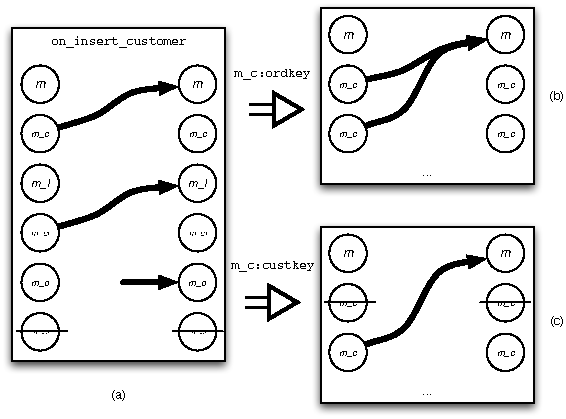
\includegraphics[width=2.5in]{graphics/MessagingGraph}
\end{center}
\caption{An example of a messaging graph based on Section \ref{sec:dbtoaster}'s example query.  (a) The messaging graph for the \texttt{on\_insert\_customer} event.  (b) The effects of splitting view $m_c$ on \texttt{ordkey}.  (c) The effects of splitting $m_c$ on \texttt{custkey}.}
\label{fig:diag:messagingGraph}
\vspace*{-0.2in}
\end{figure}

For example, consider the transition function that results from an update to the
customer table.  One specific subtask of this transition reads $m_c$ and writes
to $m$.  Treating each view as a node, this task has one edge with one read node
and one write node.

DBToaster considers database layout in terms of how it partitions data across a
physical medium (i.e., memory, disk pages, or a cluster).  Viewed through the
messaging graph, a partitioning is an assignment of all nodes in the graph to
one (or more, in the case of replication) partition.  For example, if they were
small enough, $m$ and $m_c$ might be placed on one disk page each.  Thus, the
subtask requires a read on one page, and an update to a second.

Subdivision of individual views is represented in the messaging graph by
splitting of graph nodes.  Of particular interest is how the new nodes interact
with the hyperedge(s) connected to the original node.  As the split occurs, a
node may stay connected to a hyperedge, the hyperedge may likewise be split, or
in some cases, only one node will remain connected (see Figure
\ref{fig:diag:messagingGraph}b,c).  DBToaster can exploit the limited range of
node split/hyperedge interactions to select an effective partitioning scheme.

For example, when partitioning $m_c$, horizontal partitioning on the value of
\texttt{ordkey} increases the number of nodes connected to the
\texttt{on\_insert\_customer} task edge, while using \texttt{custkey} does not
provoke an increase.  If the data represented by these nodes is split across
multiple disks or servers, the computation must still access all of them.  The
roles are reversed for the \texttt{on\_insert\_order} task edge.  Under (the
false) assumption that both insert events occur with identical frequency,
DBToaster can partition on both keys to minimize the number of connected nodes.

Additional knowledge about the dataset enhances the messaging graph produced by
DBToaster.  For instance, the E-R diagram can be integrated into the messaging
graph; the chain of foreign key dependencies in $q$ is strictly hierarchical. 
DBToaster uses this information and creates partitions along a single axis with
a secondary index to bound the number of partitions accessed by each update
subtask, with respect to the total number of partitions generated.  Similarly,
this information is used by DBToaster to select a partitioning scheme that
places nodes typically connected by a subtask into a single partition; this is
analagous to co-clustering in a traditional DBMS.


% \begin{itemize}
% \item Motivation:
%   \begin{itemize}
%   \item we've talked about incremental evaluation, from a main mem perspective
%   \item classical dbms maintains db schema in terms of processing queries over the entire data set, i.e. scans of whole tables and indexes built on whole tables
%   \item a ddms should configure the storage layer to best service updates
%   \item we look at this in terms of the auxiliary structures, and their relationship
%   \item one idea here is how to cocluster the auxiliary structures, which exploits locality
%     \begin{itemize}
%     \item in particular an update only touches a few entries in the auxiliary structure, coclustering places these entries together for efficient access to storage
%     \item another is to stripe the data to yield high aggregate bandwidth
%     \end{itemize}
%   \end{itemize}
% 
% \item Disk layout
%   \begin{itemize}
%   \item Single Disk - Cluster within disk
%   \item Multi-Disk - Stripe across disks
%   \item Distributed - Network-bound
%   \end{itemize}
% 
% \item Challenges to Partitioning
% Number of edges in dataflow graph created by a single split (ie: splitting along a particular axis with a particular program creates one-one edges, one-many edges, many-many edges) (partitioning on an output variable on right, both, or neither)
% 
% \item Indexing
%   \begin{itemize}
%   \item incrementally computing the sort order
%   \item partial indexing
%   \item update chunks (separate area that is cheap to update, i.e. no split/rebalancing of index, lazily pushed into index)
%   \end{itemize}
% \end{itemize}


\section{Discussion and Conclusions}






\end{document}
